\documentclass{beamer}
\usepackage{tikz}
\usepackage{bm}
\usepackage{amsmath}
\usepackage{amssymb}
\usepackage{amsfonts}
\usepackage{mathtools} %pro \dcases
\usepackage{tcolorbox}
\usepackage{lipsum}
\usepackage{tikz}
\usepackage{braket}
\usepackage{bbm}

\newcommand{\Subitem}[1]{\setlength\itemindent{15pt}}

\usetikzlibrary{arrows} 
%%% This file contains definitions of various useful macros and environments %%%
%%% Please add more macros here instead of cluttering other files with them. %%%

%%% Minor tweaks of style

% These macros employ a little dirty trick to convince LaTeX to typeset
% chapter headings sanely, without lots of empty space above them.
% Feel free to ignore.
\makeatletter
\def\@makechapterhead#1{
  {\parindent \z@ \raggedright \normalfont
   \Huge\bfseries \thechapter. #1
   \par\nobreak
   \vskip 20\p@
}}
\def\@makeschapterhead#1{
  {\parindent \z@ \raggedright \normalfont
   \Huge\bfseries #1
   \par\nobreak
   \vskip 20\p@
}}
\makeatother

% This macro defines a chapter, which is not numbered, but is included
% in the table of contents.
\def\chapwithtoc#1{
\chapter*{#1}
\addcontentsline{toc}{chapter}{#1}
}

% Draw black "slugs" whenever a line overflows, so that we can spot it easily.
\overfullrule=1mm

%%% Macros for definitions, theorems, claims, examples, ... (requires amsthm package)

\theoremstyle{plain}
\newtheorem{thm}{Theorem}
\newtheorem{hypot}{Hypotheses}
\newtheorem{lemma}[thm]{Lemma}
\newtheorem{definition}{Definition}

\theoremstyle{plain}
\newtheorem{defn}{Definition}

\theoremstyle{remark}
\newtheorem*{cor}{Corollary}
\newtheorem{conjecture}{Conjecture}
\newtheorem*{rem}{Remark}
\newtheorem*{example}{Example}

%%% An environment for proofs

\newenvironment{myproof}{
  \par\medskip\noindent
  \textit{Proof}.
}{
\newline
\rightline{$\qedsymbol$}
}

%%% An environment for typesetting of program code and input/output
%%% of programs. (Requires the fancyvrb package -- fancy verbatim.)

\DefineVerbatimEnvironment{code}{Verbatim}{fontsize=\small, frame=single}


%%% Useful operators for statistics and probability
\DeclareMathOperator{\sign}{\textrm{sign}}
\renewcommand{\Im}{\textrm{Im}}
\newcommand{\Par}{\textrm{par}}

%%% Transposition of a vector/matrix
\newcommand{\T}[1]{#1^\top}

%%% Various math goodies
\newcommand{\maon}[1]{o(n^{#1})}
\newcommand{\abs}[1]{\left|{#1}\right|}
\newcommand{\isqr}[1]{\frac{1}{\sqrt{#1}}}

%%% Various table goodies
\newcommand{\pulrad}[1]{\raisebox{1.5ex}[0pt]{#1}}
\newcommand{\mc}[1]{\multicolumn{1}{c}{#1}}

\DeclareMathOperator{\Tr}{\textrm{Tr}}
\DeclareMathOperator\arctanh{arctanh}
\renewcommand{\d}{\ensuremath{\mathrm{d}}}
\newcommand{\D}{\ensuremath{\mathrm{D}}}
\newcommand{\pder}[2]{\frac{\partial #1}{\partial #2}}
\newcommand{\der}[2]{\frac{\mathrm{d} #1}{\mathrm{d} #2}}
\newcommand{\Der}[2]{\frac{\mathrm{D} #1}{\mathrm{d} #2}}

\newcommand{\M}{\mathcal{M}}
\renewcommand{\P}{\mathcal{P}}
\newcommand{\R}{\mathbb{R}}
\newcommand{\N}{\mathbb{N}}
\newcommand{\F}{\mathcal{F}}
\renewcommand{\T}{\mathbb{T}}
\newcommand{\TT}{\mathcal{T}}
\renewcommand{\O}{\mathcal{O}}

\newcolumntype{L}[1]{>{\raggedright\let\newline\\\arraybackslash\hspace{0pt}}m{#1}}
\newcolumntype{C}[1]{>{\centering\let\newline\\\arraybackslash\hspace{0pt}}m{#1}}
\newcolumntype{R}[1]{>{\raggedleft\let\newline\\\arraybackslash\hspace{0pt}}m{#1}}


\newcommand{\A}{\mathcal{A}}
\newcommand{\Id}{\mathbbm{1}}
\newcommand{\llambda}{{\bm\lambda}}
\renewcommand{\AA}{\mathcal{\widehat{A}}}
\newcommand{\U}{\hat{U}}
\renewcommand{\H}{\mathcal{H}}
\newcommand{\HH}{\hat{H}}
\newcommand{\J}{\hat{J}}
\newcommand{\kpsi}{\ket{\psi}}
\newcommand{\kphi}{\ket{\phi}}
\newcommand{\kpsit}{\ket{\psi(t)}}
\newcommand{\kpsilt}{\ket{\psi(\llambda(t))}}
\newcommand{\up}{\ket{\uparrow}}
\newcommand{\dn}{\ket{\downarrow}}
\newcommand{\ch}{\hat{\chi}}
\newcommand{\Schrodinger}{Schrödinger }
\newcommand{\PH}{\mathcal{PH}}
\newcommand{\Z}{\mathbb{Z}}
\newcommand{\Span}{\text{Span}}
\renewcommand{\Re}{\text{Re}}
\newcommand{\FM}{\mathcal{FM}}

\newcommand{\expsm}{e^{-\frac{i \omega}{2}\hat\sigma_y  t}}
\newcommand{\expsp}{e^{\frac{i \omega}{2}\hat\sigma_y  t}}
\newcommand{\UU}{\hat U}


\DeclareMathOperator{\spec}{\sigma}





\usepackage{xcolor}
\definecolor{red}{rgb}{0.9,0.05,0.05}
\definecolor{redd}{rgb}{0.7,0.1,0.1}
\definecolor{reddd}{rgb}{0.7,0.2,0.0}

\definecolor{green}{rgb}{0.05,0.9,0.05}
\definecolor{greenn}{rgb}{0.2,0.65,0.2}
\definecolor{greennn}{rgb}{0.2,0.8,0.7}

\definecolor{blue}{rgb}{0.05,0.05,0.9}
\definecolor{bluee}{rgb}{0.2,0.2,0.6}
\definecolor{blueee}{rgb}{0.7,0.6,0.9}


\newcommand{\red}[1]{\textcolor{red}{#1}}
\newcommand{\redd}[1]{\textcolor{redd}{#1}}
\newcommand{\reddd}[1]{\textcolor{reddd}{#1}}

\newcommand{\green}[1]{\textcolor{green}{#1}}
\newcommand{\greenn}[1]{\textcolor{greenn}{#1}}
\newcommand{\greennn}[1]{\textcolor{greennn}{#1}}

\newcommand{\blue}[1]{\textcolor{blue}{#1}}
\newcommand{\bluee}[1]{\textcolor{bluee}{#1}}
\newcommand{\blueee}[1]{\textcolor{blueee}{#1}}

\newcommand{\gray}[1]{\textcolor{gray}{#1}}



\newcommand{\leftsquigarrow}{\reflectbox{$\rightsquigarrow$}}
\newcommand{\curlyrightarrow}[1]{\overset{\rightsquigarrow}{#1}}
\newcommand{\curlyleftarrow}[1]{\overset{{\leftsquigarrow}}{#1}}
\setbeamercolor{block title}{bg=blue!4,fg=black}

\newcommand*{\defeq}{\mathrel{\vcenter{\baselineskip0.5ex \lineskiplimit0pt
                     \hbox{\scriptsize.}\hbox{\scriptsize.}}}=}
\DeclareMathOperator\arctanh{arctanh}
\newcommand{\abs}[1]{\left|{#1}\right|}
\addtobeamertemplate{navigation symbols}{}{%
    \usebeamerfont{footline}%
    \usebeamercolor[fg]{footline}%
    \hspace{1em}%
    \insertframenumber/17%\inserttotalframenumber
}
\begin{document}

\titlegraphic{
\includegraphics[width=0.8\textwidth]{pics/mff_cz_color.pdf}}
\title{Geometrický přístup k externě vedeným kvantovým systémům}   
\author{\textbf{Bc. Jan Střeleček} \\ vedoucí práce: \textbf{prof. RNDr. Pavel Cejnar, Dr., DSc.}\\ Ústav částicové a jaderné fyziky}
\date{16.5.2022} 

\frame{\titlepage} 

% \frame{
%   \frametitle{Motivace}
%   \framesubtitle{Proč nás zajímají Hamiltoniány s parametrem?}

% \begin{block}{Adiabatické kvantové počítání}
% \begin{enumerate}
%   \item Systém lze snadno připravit do počátečího stavu.
%   \item Metodou \emph{kvantového annealingu} je systém převeden do superpozice reprezentující matematickou úlohu.
%   \item Systém je zkolabován do stavu s lokálně nejnižší energií.
%   \item Proces se opakuje, dokud není nalezena celková nejnižší energie. Příslušný vlastní vektor reprezentuje výsledek úlohy.
% \end{enumerate}
% \begin{figure}
%   \centering
%   \begin{tikzpicture}
%     \node[] at (0,0) {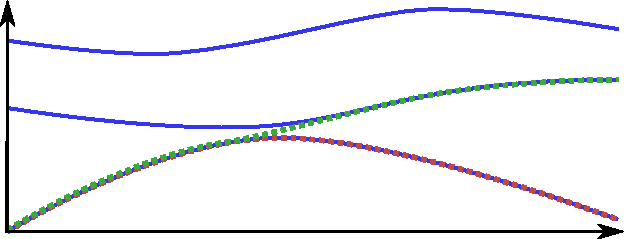
\includegraphics[width=0.6\textwidth]{../dp_text/img/introDriving.pdf}};
%     \node[] at (-3.2,1.6) {$\blue E$};
%     \node[] at (3.3,-1.3) {$t$};
%   \end{tikzpicture}
% \end{figure}
% \end{block}
% }

\frame{
  \frametitle{Geometrie problému}
  \framesubtitle{Které kvantové struktury je výhodné popisovat geometricky a proč to dělat?}

  \begin{block}{Hamiltonian s parametrem $\HH(\llambda)$ pro $\llambda\in\R^n$}
    \begin{itemize}
      \item změna $\llambda$ \emph{řídí} kvantový stav 
      \item po měření stav kolabuje do vl. stavu pro aktuální parametr $\llambda$
    \end{itemize}
  \end{block}
\vspace{20pt}
  \begin{block}{Využití}
    \begin{itemize}
      \item kvantové počítače ($\llambda$ je síla interakce mezi qubity)
      \item biologické struktury (např. fotosyntéza)
    \end{itemize}
  \end{block}
  % \begin{block}{Stavová varieta}
  %   \begin{equation}
  %     \M_s\coloneqq \left\{\bigcup_{\varphi\in[0,2\pi)} \bigcup_{\llambda\in\mathcal U} e^{i\varphi}\ket{s(\llambda)}\right\}.
  %   \end{equation}
  % \end{block}
}

% \frame{
%   \frametitle{Geometrie problému}

%   \begin{figure}[h]
%     \centering
%     % 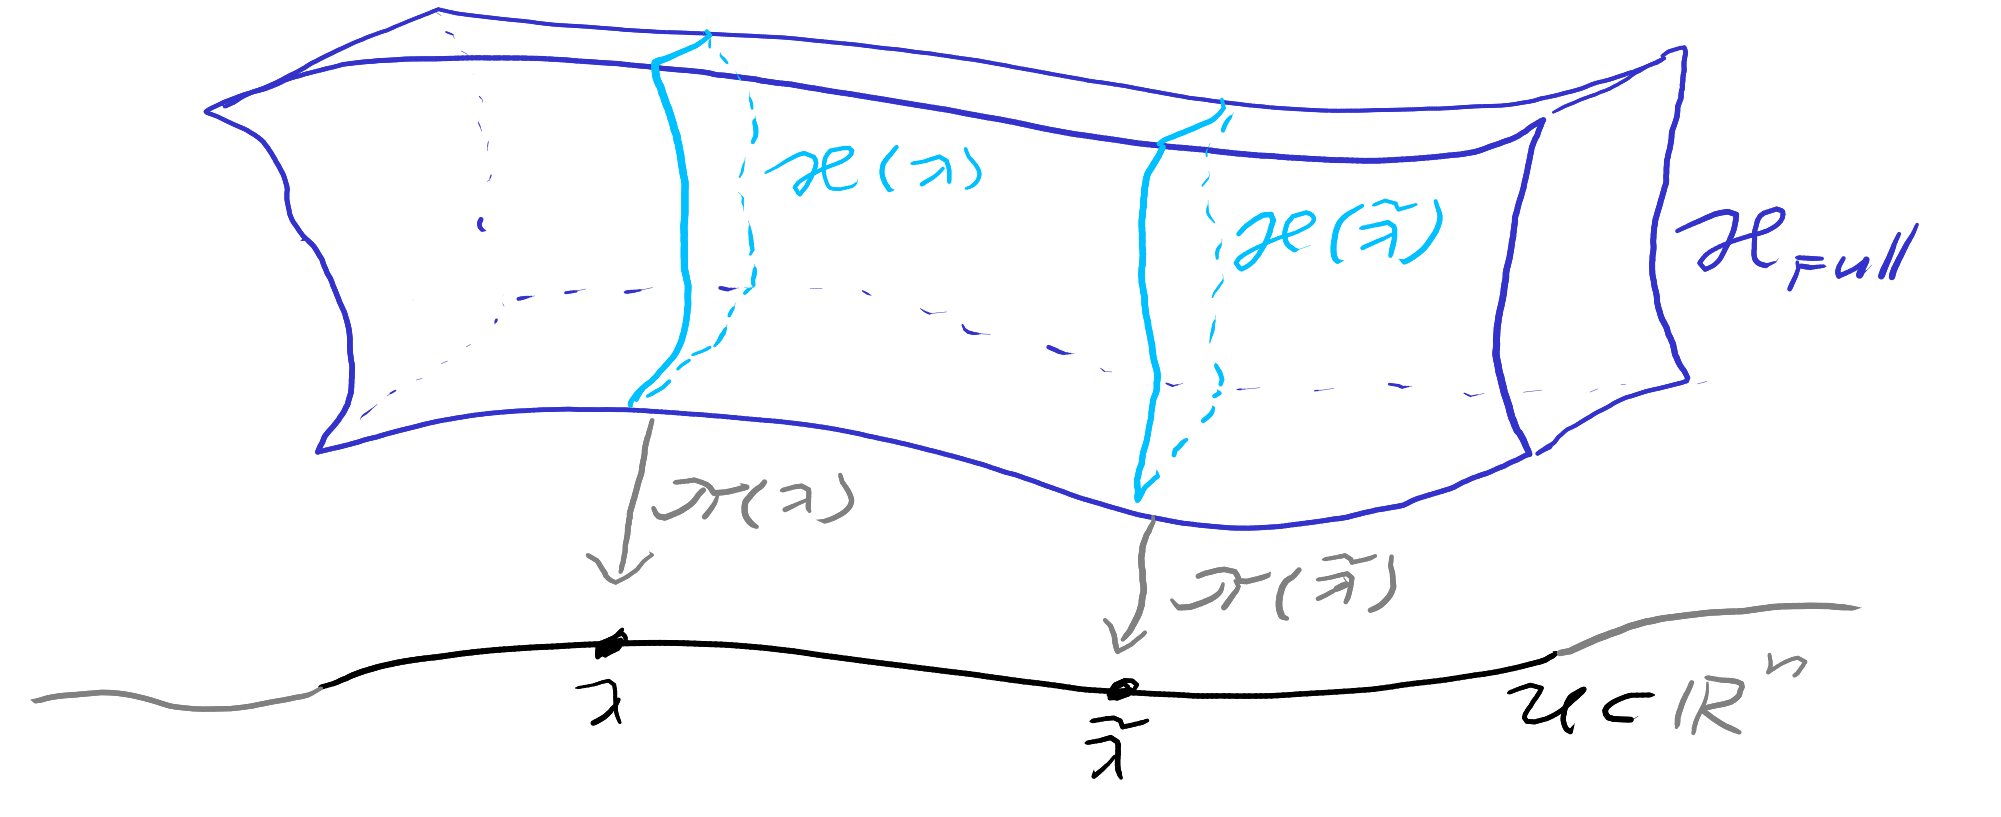
\includegraphics[width=\textwidth]{../img/manifold_basic_1.png}
%     \begin{tikzpicture}
%         \node[] at (0,0) {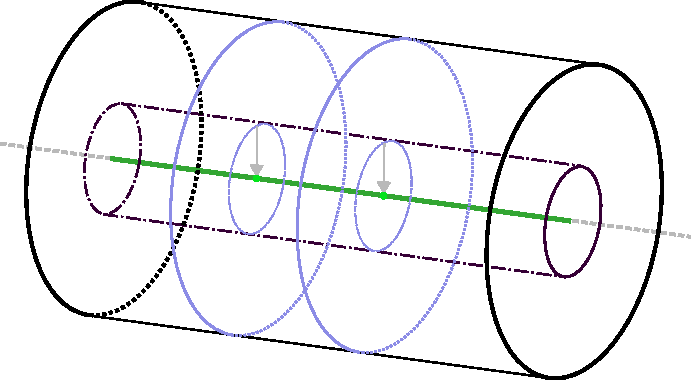
\includegraphics[width=0.7\textwidth]{../dp_text/img/fullHilbert.pdf}};
%         \node[] at (3.0,-0.2) {$\greenn{\mathcal U}$};
%         \node[] at (4.6,-0.7) {$\gray{\R^n}$};
%         \node[] at (2.8,1.8) {$\H_{full}$};
%         \node[] at (-0.5,2) {$\blueee{\H(\llambda)}$};
%         \node[] at (1.0,1.83) {$\blueee{\H(\tilde\llambda)}$};
%         \node[] at (-0.8,0.95) {$\gray{\pi(\llambda)}$};
%         \node[] at (0.8,0.75) {$\gray{\pi(\tilde\llambda)}$};
%         \node[] at (-1,-0.17) {\green{$\llambda$}};
%         \node[] at (0.4,-0.4) {\green{$\tilde\llambda$}};
%     \end{tikzpicture}
% \vspace{-3pt}
% \caption{Base manifold $\greenn{\mathcal U}\subset \gray{\R^n}$. For every point $\green\llambda\in\greenn{\mathcal U}$ one \bluee{Hilbert space $\H(\llambda)$} is constructed as a \bluee{fiber}.}
%     \label{fig:wholeBundle}
% \end{figure}

% }

\frame{
  \frametitle{Geometrie problému}


  \vspace{-15pt}\begin{figure}[h]
    \centering
    % 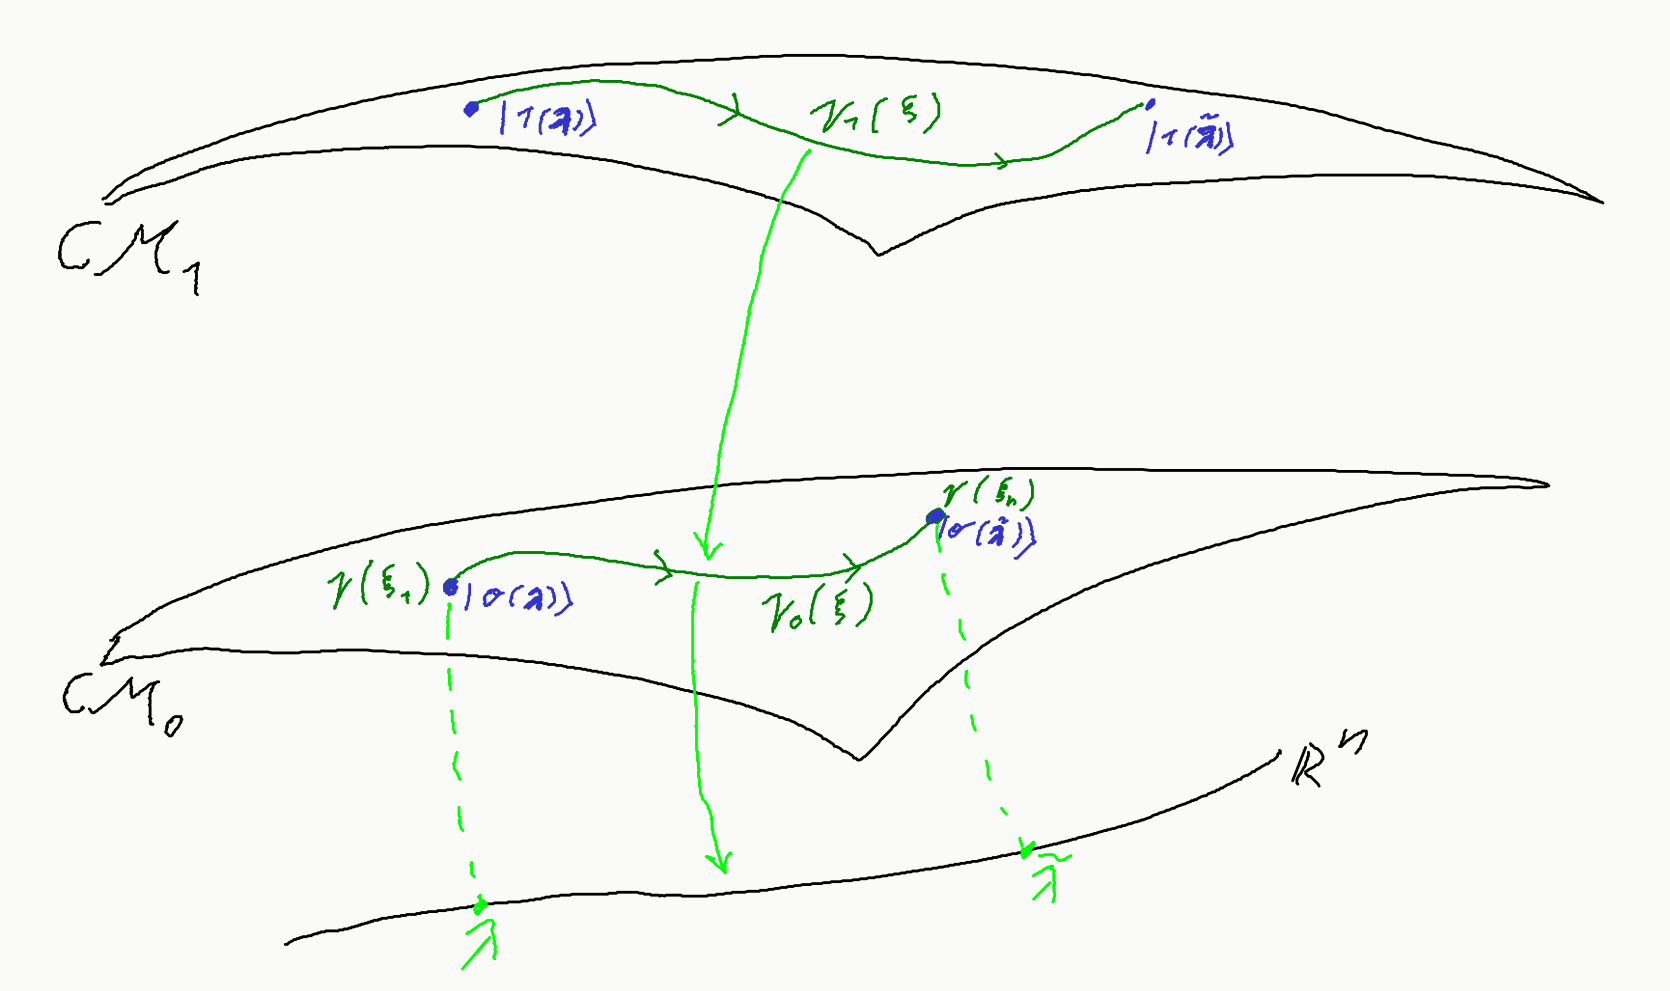
\includegraphics[width=\textwidth]{../img/manifoldCutIntuition.png}
        \begin{tikzpicture}
        \node[] at (0,0) {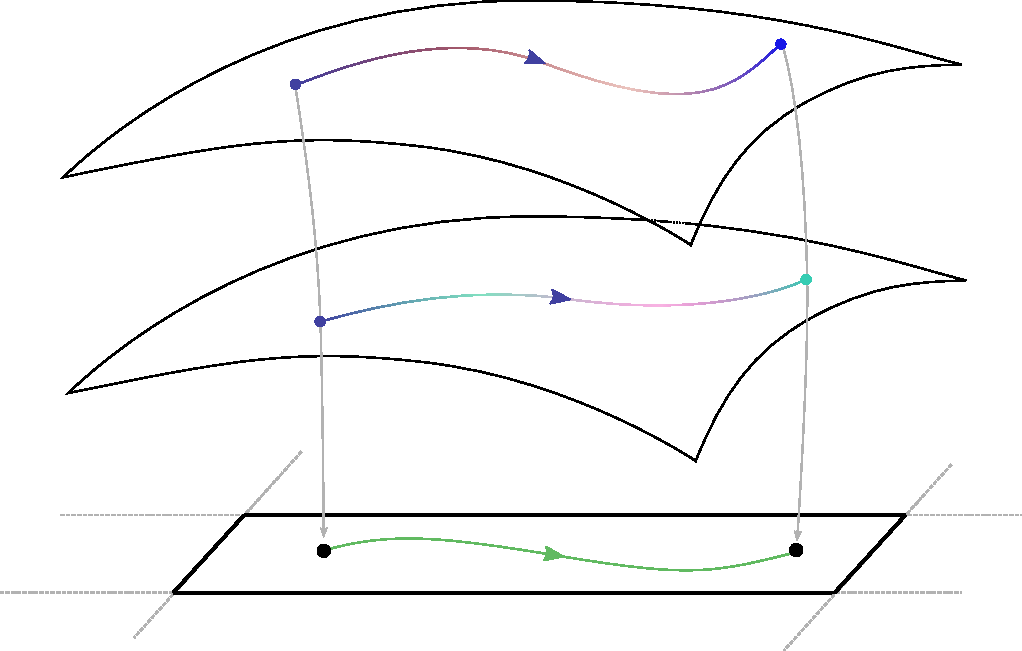
\includegraphics[width=0.9\textwidth]{../dp_text/img/manifold_structure.pdf}};
        \node[] at (3.7,-2.7) {$\mathcal U\subset \gray{\R^n}$};
        \node[] at (-4.2,-1.0) {$\M_0$};
        \node[] at (-4.2,1.1) {$\M_1$};
        \node[] at (-2.6,2.0) {$\bluee{\ket{1(\llambda)}}$};
        \node[] at (3.2,2.7) {$\blue{\ket{1(\tilde\llambda)}}$};
        \node[] at (-2.4,-0.0) {$\bluee{\ket{o(\llambda)}}$};
        \node[] at (3.4,0.5) {$\greennn{\ket{o(\tilde\llambda)}}$};
        \node[] at (-1.3,-2.34) {$\llambda=\greenn{\mathcal J(0)}$};
        \node[] at (3.7,-2.25) {$\tilde\llambda=\greenn{\mathcal J(T)}$};
        \node[] at (1.2,-2.1) {$\greenn{\mathcal J(t)}$};
        \node[] at (-1.1,-0.8) {$\gray{\pi(\llambda)}$};
        \node[] at (3.3,-0.8) {$\gray{\pi(\tilde \llambda)}$};
    \end{tikzpicture}
  \end{figure}
  \vspace{-15pt}
\begin{block}{Základní stavová varieta}
  \vspace{-10pt}\begin{equation}
    \M_0\coloneqq \left\{\bigcup_{\varphi\in[0,2\pi)} \bigcup_{\llambda\in\mathcal U} e^{i\varphi}\ket{0(\llambda)}\right\}.
  \end{equation}
\end{block}
}

\frame{
  \frametitle{Geometrie stavových variet}

 \begin{block}{Metrický tensor na stavových varietách}
    \vspace{-22pt}\begin{equation}
        \begin{split}
            g_{\mu\nu}&: \redd{\mathbb T\mathcal U}\times \redd{\mathbb T\mathcal U}\rightarrow \R \\
            g_{jk}\redd{\d \bm \lambda^j \d\bm \lambda^k}+\O(\lambda^3) \equiv \d s^2 &\coloneqq 1-\underbrace{\left|\braket{o(\bm\llambda+\delta\bm\llambda)|o(\bm\llambda)}\right|^2}_{F(\bm\llambda+\delta\bm\llambda,\bm\llambda)}.
        \end{split}
    \end{equation} 

    \vspace{-5pt}{Na k-té stavové varietě lze ukázat:}
    \begin{equation}
      g_{\mu\nu}^{(k)} = \Re \sum_{j\neq k}\frac{\braket{k|\pder{\HH(\llambda)}{\lambda^\mu}|j}\braket{j|\pder{\HH(\llambda)}{\lambda^\nu}|k}}{(E_k-E_j)^2}.
    \end{equation}
  \end{block}
\begin{block}{Fidelita}
  \begin{itemize}
    \item pro čisté stavy: $F: \H\times\H\mapsto [0;1]$,\quad $F(\ket{\rho},\ket{\sigma}) = \left| \braket{\rho|\sigma}\right|^2$
    \item při drivingu na stavové varietě: pravděpodobnost neexcitace
    \item Infidelita $\equiv F^*\coloneqq 1-F$
  \end{itemize}
\end{block}
}


\frame{
  \frametitle{Řízení kvantových systémů (state driving)}
  \framesubtitle{Jak výhodně (aniž by excitovaly) transportovat stavy?}

Snaha dosáhnout co nejvyšší fidelity ($F=1$)
  \begin{itemize}
      \item téměř adiabatický transport — pomalá změna parametru $\llambda$
      \item variace trajektorie — malé $\Delta E$ znamená snížení fidelity transportu
      \item counter-diabatické řízení — excitaci lze zamezit opravou Hamiltoniánu (teorie kalibračních polí)
  \end{itemize}

  \begin{figure}
    \centering
    \begin{tikzpicture}
      \node[] at (0,0) {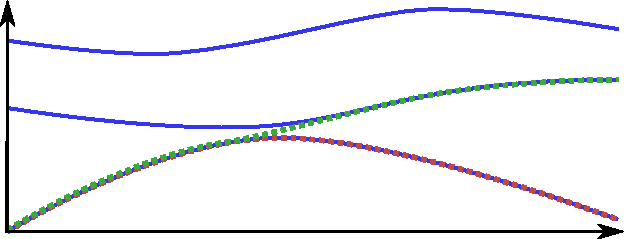
\includegraphics[width=0.6\textwidth]{../dp_text/img/introDriving.pdf}};
      \node[] at (-3.2,1.6) {$\blue E$};
      \node[] at (3.3,-1.3) {$t$};
    \end{tikzpicture}
  \end{figure}

}


\frame{
  \frametitle{Dvouhladinový systém (toy model)}
  \framesubtitle{Poznatek \#1: Fidelita se chová jako harmonický oscilátor.}
  \begin{equation}
    \HH(t)=\begin{pmatrix}
        \Omega(t)&\Delta(t)\\
        \Delta(t)&-\Omega(t)
    \end{pmatrix}
\end{equation}
\begin{equation}
  \HH(t)\ket{\psi(t)}=i\frac{\d}{\d t}\ket{\psi(t)}; \quad 
  \ket{\psi(t)}\eqqcolon \begin{pmatrix}
       a(t) \\
       b(t)    
  \end{pmatrix}
\end{equation}
\begin{equation}
  \begin{pmatrix}
    a(0)\\b(0)
  \end{pmatrix}=\ket{0(0)}
\end{equation}

\begin{block}{Řešení}
  \vspace{-25pt}
  \begin{align}
    0&= \ddot a(t)+ \gamma(t) \dot a(t)+\omega^2(t)a(t)\\
    \gamma(t)&\coloneqq -\frac{\dot \Delta(t)}{\Delta(t)}\\
    \omega^2(t) &\coloneqq i\left(\dot \Omega(t)-\frac{\dot\Delta(t)}{\Delta(t)}\Omega(t)\right)+\Delta^2(t)+\Omega^2(t)
  \end{align}
\end{block}
}



% \frame{
%   \frametitle{Dvouhladinový systém (toy model)}
%   \framesubtitle{Poznatek \#1: Existují výjimečné finální časy, pro které je $F=1$}
  
%   \begin{figure}[h]
%     \centering
%     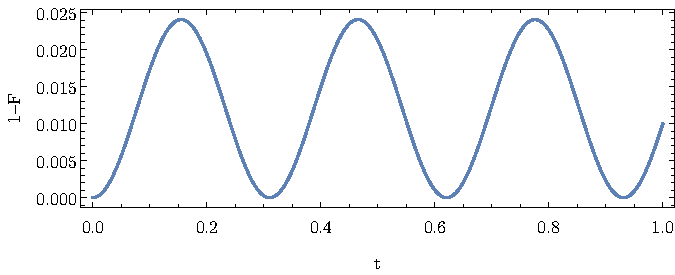
\includegraphics[scale=0.9]{../dp_text/img/infidelityTimePlotGeod.pdf}
%     \caption{Infidelita v čase pro finální čas $T=1$, geodetický driving.}
%   \label{fig:infidelityTimePlot}
% \end{figure}
% }
% \frame{
%   \frametitle{Dvouhladinový systém (toy model)}
%   \framesubtitle{Poznatek \#1: Existují výjimečné finální časy, pro které je $F=1$}
  
%   \begin{figure}[h]
%     \centering
%     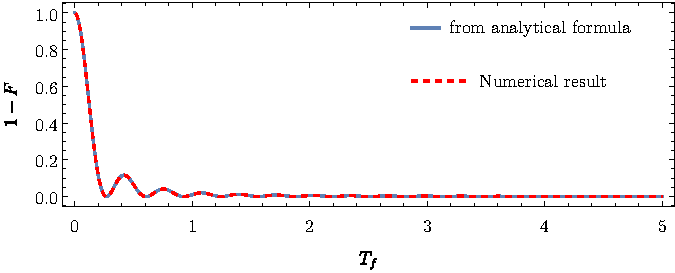
\includegraphics[scale=0.8]{../dp_text/img/infidelityTfPlot.pdf}
% \end{figure}
% \vspace{-20pt}\begin{figure}[h]
%   \centering
%   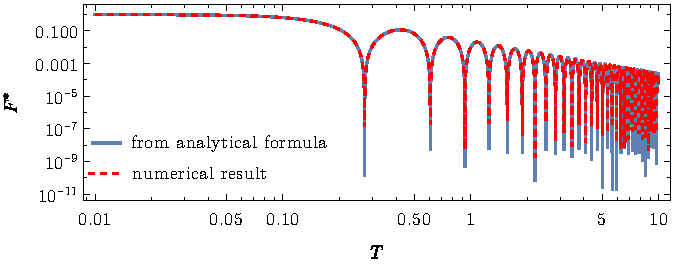
\includegraphics[scale=0.8]{../dp_text/img/infidelityTfPlotLog.pdf}
% \end{figure}

% }


\frame{
  \frametitle{Dvouhladinový systém (toy model)}
  \framesubtitle{Lineární driving}
  \qquad\qquad\qquad\qquad\qquad\qquad\qquad\qquad\qquad\qquad\qquad$\Delta E$
  \vspace{-10pt}\begin{figure}[h]
    \centering
    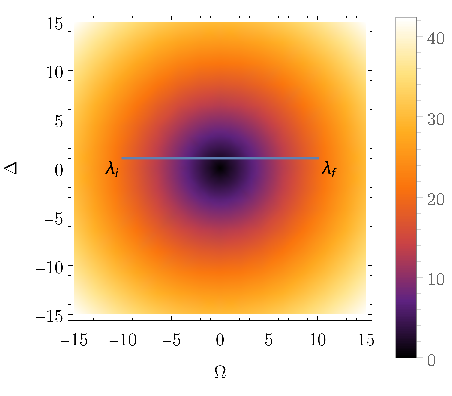
\includegraphics[scale=1.]{../dp_text/img/drivingLin.pdf}
\end{figure}
}
\frame{
  \frametitle{Dvouhladinový systém (toy model)}
    \framesubtitle{Poznatek \#2: přiblížení energetických hladin tvoří kmity, existuje \emph{kritický finální čas}}
\vspace{-30pt}\begin{figure}[h]
    \centering 
    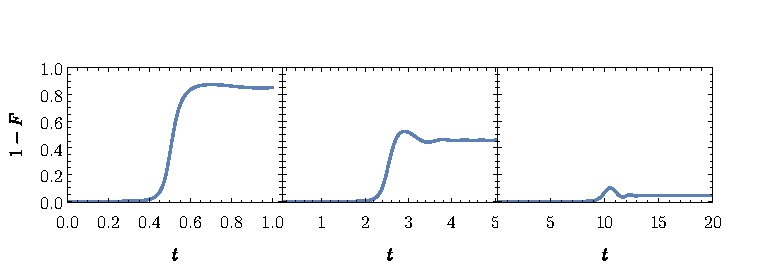
\includegraphics[scale=0.9]{../dp_text/img/infidelityInTimePlot1.pdf}
\end{figure}

\vspace{-20pt}\begin{figure}[h]
  \centering
  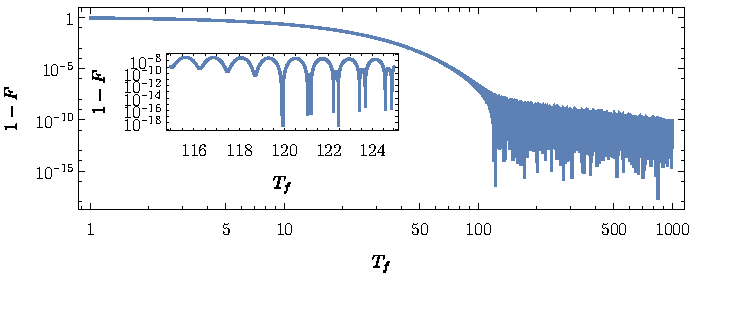
\includegraphics[scale=0.9]{../dp_text/img/infidelityTfPlotLogLinCombined1.pdf}
\end{figure}

}

\frame{
  \frametitle{Dvouhladinový systém (toy model)}
    \framesubtitle{Poznatek \#3: Kritický finální čas je v bodě, kdy oscilace nabývají $F^*=0$}
  \begin{figure}[h]
      \centering
      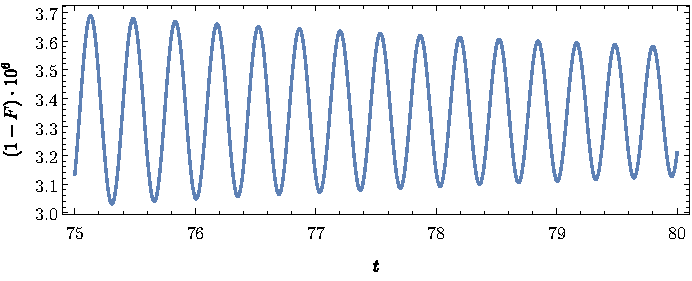
\includegraphics[scale=0.75]{../dp_text/img/undercritical.pdf}
  \end{figure}
  
  \vspace{-15pt}\begin{figure}[h]
      \centering
      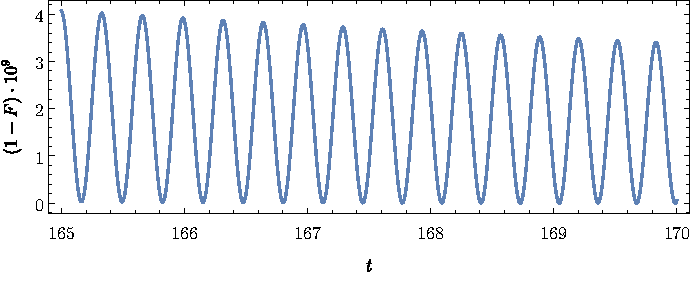
\includegraphics[scale=0.75]{../dp_text/img/overcritical.pdf}
      \vspace{-10pt}\caption{$T=80<T_c$ (nahoře), $T=170>T_c$ (dole)}
  \end{figure}
}

\frame{
  \frametitle{Dvouhladinový systém (toy model)}
    \framesubtitle{Poznatek \#4: Landau-Zener a adiabatická perturbační teorie}
    \begin{figure}[h]
      \centering 
      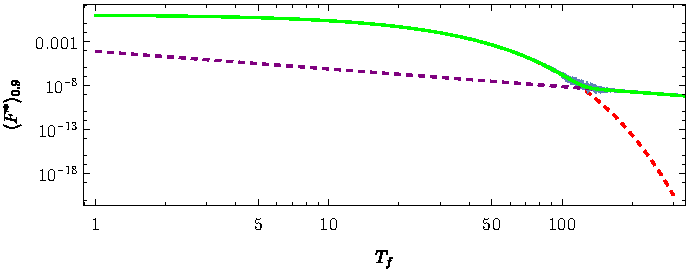
\includegraphics[scale=0.8]{../dp_text/img/landauCompare.pdf}
\caption{Zhlazená finální infidelita v závislosti na finálním čase, popsaná \green{součtem} of \red{Landau-Zenerovy rovnice} a \textcolor{purple}{adiabatickou perturbační teorií}.}
      \label{fig:landauCompare}
  \end{figure}

}

% \frame{
%   \frametitle{Dvouhladinový systém (toy model)}
%     \framesubtitle{Poznatek \#4: Landau-Zener a adiabatická perturbační teorie}
% \begin{block}{Landau-Zener-Stueckelberg (LZS) pro lineární driving}
%   Pro 
%   \begin{itemize}
%       \item dvouhladinový hamiltonian
%       \item s degenerací pouze v jednom bodě,
%       \item pro lineární křivku v parametrickém prostoru,
%   \end{itemize}
%   lze fidelitu pro fináltní časy $T\in(0,T_c)$ popsat, jako
%   \begin{equation}
%       F_T = \exp\left(-\frac{2 \pi A^2}{v|\Delta F|}\right),
%       \label{eq:exponentialPart}
%   \end{equation}
%   pro \emph{diabatický coupling} $A$ a \emph{diabatický potenciálový rozdíl} $|\Delta F|$. 
% \end{block}

% }



% \frame{
%   \frametitle{Dvouhladinový systém (toy model)}
%     \framesubtitle{Poznatek \#3: Kritický finální čas je v bodě, kdy oscilace nabývají $F^*=0$}
%     \begin{figure}[h]
%       \centering 
%       \vspace{-2pt}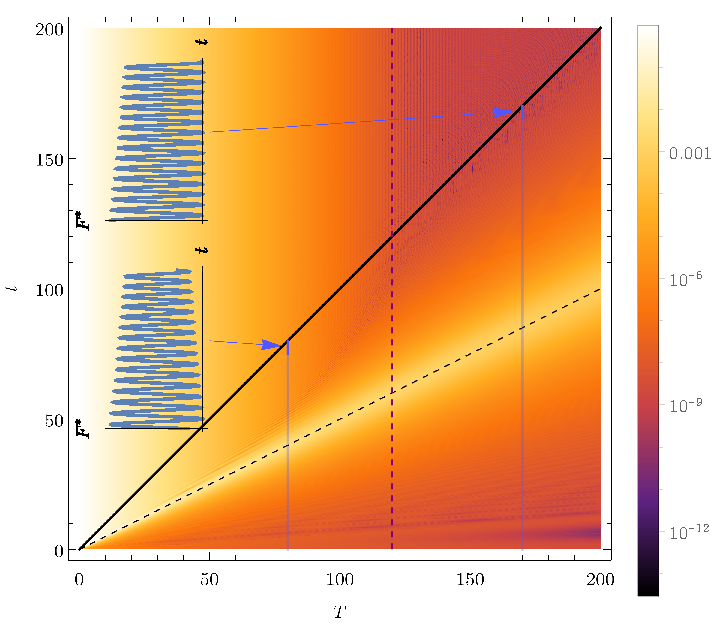
\includegraphics[scale=0.6]{../dp_text/img/allInOne.pdf}
%       \vspace{-17pt}\caption{Závislost Infidelity pro lineární driving při $\Delta=1$. Černá čára značí $t=T$, čárkovaně je vyznačen $t=T/2$, \redd{červená} čárkovaná čára je přibližná hodnota $T_c$. \bluee{Modře} jsou vyznačeny infidelity ke konci drivingu.}
%       \label{fig:AllInOne}
%   \end{figure}
% }


\frame{
  \frametitle{Lipkin-Meshkov-Glick model}
  \framesubtitle{Jak vypadá řízení v mnohočásticovém, zcela propojeném systému qubitů?}
  
  \begin{equation}
    \HH(\lambda,\chi)=\J_3+\lambda\hat V_1 +\chi \hat V_2+\chi^2 \hat V_3,
    \label{eq:firstOrderTransitionHamiltonian}
\end{equation}
pro
\begin{align}
    \hat V_1 &\coloneqq-\frac{1}{2j}\J_1^2\\
    \hat V_2 &\coloneqq -\frac{1}{2j}\left[\J_1(\J_3+j\Id)+(\J_3+j\Id)\J_1\right]\\
    \hat V_3 &\coloneqq -\frac{1}{2j}(\J_3+j\Id)^2,
\end{align}
a \emph{operátor momentu hybnosti} $\bm\J=(\J_1,\J_2,\J_3)^T$. Zvolíme $j=N/2$.
}


% \frame{
%   \frametitle{Lipkin-Meshkov-Glick model}
%   \framesubtitle{$N=3$}
%   Pentadiagonální maticová reprezentace (baze sférických harmonických funkcí $\ket{j,m}$).
%   \begin{equation}
%     \HH=\left(
%         \begin{array}{cccc}
%          -\frac{ \lambda +6}{4} & -\frac{\chi }{2 \sqrt{3}} & -\frac{\lambda }{2 \sqrt{3}} & 0 \\
%          -\frac{\chi }{2 \sqrt{3}} & \frac{ \left(-7 \lambda -4 \chi ^2-6\right)}{12} & -\chi  & -\frac{\lambda }{2 \sqrt{3}} \\
%          -\frac{\lambda }{2 \sqrt{3}} & -\chi  & \frac{ \left(-7 \lambda -16 \chi ^2+6\right)}{12} & -\frac{5 \chi }{2 \sqrt{3}} \\
%          0 & -\frac{\lambda }{2 \sqrt{3}} & -\frac{5 \chi }{2 \sqrt{3}} & -\frac{\lambda }{4}-3 \chi ^2+\frac{3}{2} \\
%         \end{array}
%         \right)
% \end{equation}
% Spektrum je degenerované, lze zapsat jako
% \begin{align}
%         E_0 &= \left(G-F-\frac{\sqrt{D-E}}{2}\right)
% ,\quad
%         E_1 = \left(G-F+\frac{\sqrt{D-E}}{2}\right)
% \\
%         E_2 &= \left(G+F-\frac{\sqrt{D+E}}{2}\right)
% ,\quad
%         E_3 = \left(G+F+\frac{\sqrt{D+E}}{2}\right)
% \end{align}

% }


\frame{
  \frametitle{Lipkin-Meshkov-Glick model}
  
  \begin{figure}[H]
    \centering
    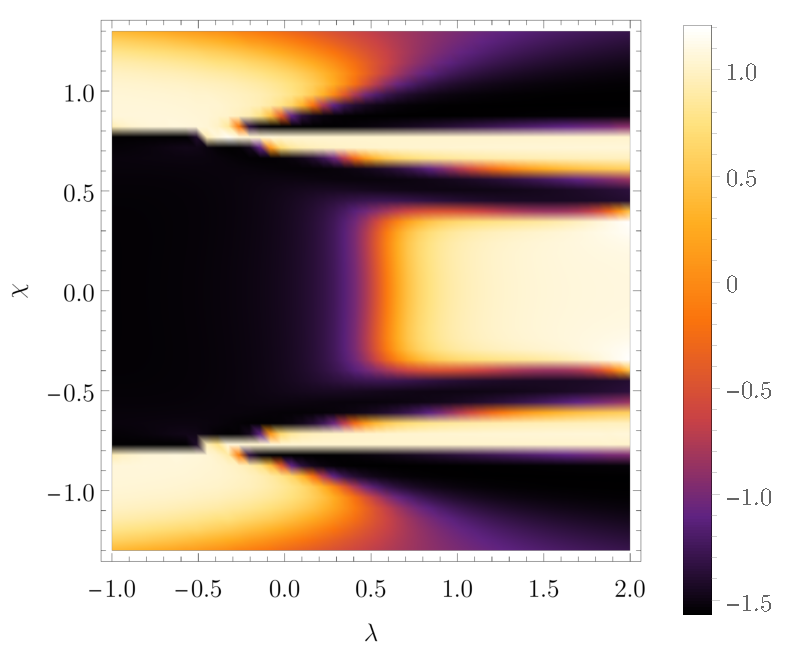
\includegraphics[scale=0.7]{../dp_text/img/N=3_Ricci.pdf}
    \vspace{-5pt}\caption{Ricciho křivost základní stavové variety pro $N=3$.}
    \label{fig:N=3_Ricci}
\end{figure}
}




\frame{
  \frametitle{Lipkin-Meshkov-Glick model}
  \begin{figure}[H]
    \centering
    % \includegraphics{../img/N=3_geodesics.pdf}
    \begin{tikzpicture}
        \node[anchor=south west,inner sep=0] at (0,0) {\includegraphics[scale=0.7]{../dp_text/img/N=3_geodesics.pdf}};
        % \draw[blueee,ultra thick] (4.5,9.56) -- (10.67,10.5);
        % \draw[blueee,ultra thick] (4.5,2.71) -- (10.67,1.8);
    \end{tikzpicture}
    \vspace{-10pt}\caption{\green{Geodetiky} pro $N=3$ z bodu $(\lambda_i;\chi_i)=(0;0)$. V pozadí $\det g$.}
    \label{fig:N=3_geodesics}    
\end{figure}
  

}




\frame{
  \frametitle{Lipkin-Meshkov-Glick model}
  \framesubtitle{}
  

  \begin{minipage}[t]{0.48\linewidth}
    \begin{equation*}
      (\lambda_{l,r} ;\pm\chi_{l,r})= \begin{cases}
          \left(1-\frac{N}{2};\sqrt{\frac{N}{N+2}}\right)\\
          \left(1-N;\sqrt{\frac{N}{N+1}}\right)
      \end{cases}
      \label{eq:singularityCoordinateFormulaLeft}
    \end{equation*}
     
    \begin{equation*}
      \text{pro } N\geq 3 \begin{cases}
        \text{liché} \\
        \text{sudé}
      \end{cases}
     \end{equation*}

     \bluee{Figure:} Degenerace vpravo jsou značeny mezi $E_0$ a $E_1$ pro dimenze 1,3,5,7 v prvním a 2,4,5,8 v druhém sloupci.
  \end{minipage}%
  \begin{minipage}[t]{0.48\linewidth}
    \begin{figure}[h]
      \centering
      \vspace{-50pt}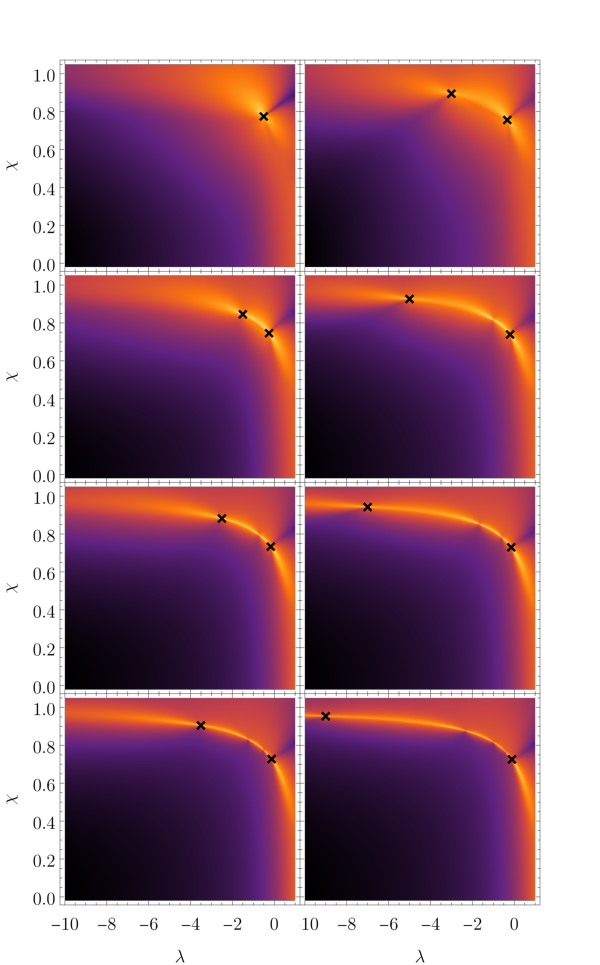
\includegraphics[scale=0.59]{../dp_text/img/singularitiesPlots.pdf}
     
  \end{figure}
  \end{minipage}


  
}





\frame{
  \frametitle{Lipkin-Meshkov-Glick model}
  \framesubtitle{Zpomalování geodetik u singularit a jejich využití -- transport pomocí \emph{quenchů}.}
  \begin{figure}[h]
    \centering
    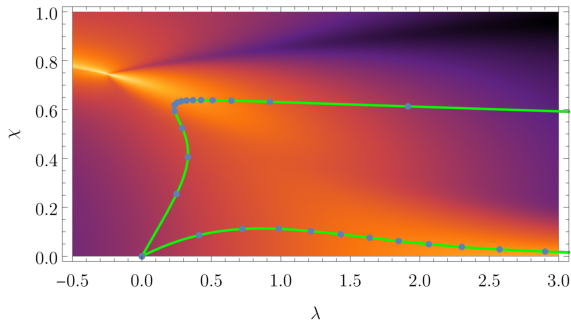
\includegraphics[scale=1.]{../dp_text/img/bg123.pdf}
    % 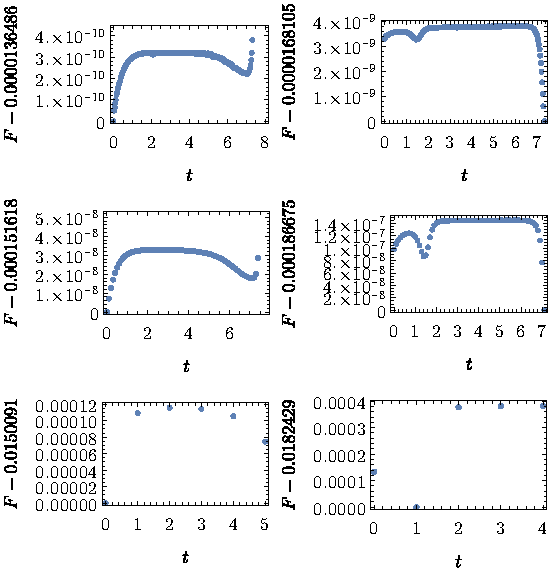
\includegraphics[scale=1.]{../dp_text/img/plotsFidelityQuenches.pdf}
    \caption{Dimenze $N=3$, 2 různé geodetiky, časový rozdíl mezi vedlejšími body $\Delta t=0.5$.}
\end{figure}
  
}

\frame{
  \frametitle{Závěr}
  \framesubtitle{Co jsme se dozvěděli a kudy dál?}
  \begin{block}{Co jsme se dozvěděli}
    
    \begin{itemize}
      \item Reformulace některých geometrických struktur v teorii 
      \item prozkoumána fidelita lineárního a geodetického drivingu ve dvouhladinovém systému
      \begin{itemize}
        \item vysvětlení oscilací a analyptické vztahy pro geodetický a lineární driving
        \item význačné body finálního času (někdy je $F=1$, vysvětlení $T_C$)
        \item aproximativní metody (\emph{Landau-Zener},\emph{adiabatická perturbační teorie})
      \end{itemize}
      \item Pro Lipkin-Meshkov-Glick model známe strukturu základní stavové veriety
      \begin{itemize}
        \item geometrické veličiny
        \item geodetiky
        \item body degenerace v závislosti na dimenzi
      \end{itemize}
    \end{itemize}
  \end{block}

}


\frame{
  \frametitle{Děkuji za pozornost}
  \framesubtitle{Nechť je zbytek Vašeho dne krásný...}

  Nejdůležitější odkazy zde:

  \textbf{M. Kolodrubetz, P. Mehta, and A. Polkovnikov}. Geometry and non-adiabatic
  response in quantum and classical systems. Physics Reports, 697:1–87, 2017.
  ISSN 0370-1573.
  
  \textbf{M. V. Berry}. Quantal phase factors accompanying adiabatic changes. Proc.
  R. Soc. Lond. A, 392(1802):45–57, 1984. doi: 10.1098/rspa.1984.0023.
  
  \textbf{M. V. Berry}. The quantum phase, five years after. A Shapere, F Wilczek.
  (World Scientific) 7-28, 1989. Geometric phases in physics, 7–28, Adv. Ser.
  Math. Phys., 5,.
  
  \textbf{M. V. Berry}. Transitionless quantum driving. Journal of Physics A: Math-
  ematical and Theoretical, 42(36), 2009. doi: 10.1088/1751-8113/42/36/
  365303.

  \dots více brzy ve článcích spolu s Pavel Cejnar, Felipe Matus a Pavel Stránský.

}


\frame{
  \begin{block}{Otázka oponenta}
    V diskusi dvouhladinového modelu mimo jiné diskutujete vedení po geodetice, ale nediskutujete
geometrii variety základního stavu, neuvádíte metrický tensor ani nedokazujete, že zvolená
trajektorie je skutečně geodetika. Bylo by možné tyto informace doplnit?
  \end{block}
}

\frame{
  \frametitle{Otázka oponenta ohledně Dvouhladinového systému}
  \framesubtitle{Důkaz, že oblouk na obrázku je geodetikou}
  \qquad\qquad\qquad\qquad\qquad\qquad\qquad\qquad\qquad\qquad\qquad$\Delta E$
  \vspace{-10pt}\begin{figure}[h]
    \centering
    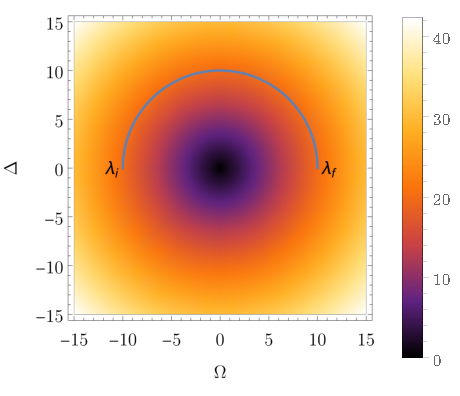
\includegraphics[scale=1.1]{../dp_text/img/driving.pdf}
\end{figure}
}

\frame{
  \frametitle{Otázka oponenta ohledně Dvouhladinového systému}
  \framesubtitle{Metrický tenzor}
  Od Hamiltonianu v souřadnicích $(\Delta(t);\Omega(t))$
  \begin{equation}
    \HH(t)=\begin{pmatrix}
        \Omega(t)&\Delta(t)\\
        \Delta(t)&-\Omega(t)
    \end{pmatrix}
  \end{equation}
  přejdeme k polárním souřadnicím $(r(t),\phi(t))$, definovaným vztahy
  \begin{align}
    \Delta (t)&= r(t)\sin \phi(t),\quad \Omega(t) = r(t)\cos \phi(t).
  \end{align}
  V nich je metrický tenzor
  \begin{equation}
    g_{\mu\nu}^{(0)}=\Re\frac{\braket{0|\partial_\mu \HH|1}\braket{1|\partial_\nu \HH|0}}{(E_1-E_0)^2}=
    \begin{pmatrix}
      0&0\\
      0&\frac{1}{4}\\  
    \end{pmatrix}.
  \end{equation}

}

\frame{
  \frametitle{Otázka oponenta ohledně Dvouhladinového systému}
  \framesubtitle{Metrický tenzor}
  Geodetickou rovnici pak splňují drivingy s $\ddot\theta=0$, tedy
  \begin{equation}
    \theta(t) = \theta_i+(\theta_F-\theta_i)\frac{t}{T}
  \end{equation}
  \begin{itemize}
    \item $\theta_i$ je počáteční úhel v čase $t=0$
    \item $\theta_T$ je finální úhel v čase $T$
  \end{itemize}

  $r(t)$ lze volit libovolně, v rámci práce byl zvolen geodetický driving $r(t)= \text{konst}$.

  \vspace{10pt}
  Třída geodetik je ale mnohem širší\dots
}

\frame{
  \frametitle{Otázka oponenta ohledně Dvouhladinového systému}
  \framesubtitle{Metrický tenzor}
  Zafixujme jednu souřadnici, $(\Delta;\Omega(t))$. Pak
  \begin{equation}
    g_{\Omega\Omega}=\frac{\Omega^2}{4(\Omega^2+\Delta^2)^2}.
  \end{equation}
  Z vlastnosti geodetiky $g_{\Omega\Omega}\dot\Omega^2=\text{konst.}$ plyne
  \begin{equation}
    \Omega(t) = \Delta \tan\Big(a_i+(a_f-a_i)\frac{t}{T}\Big);\quad a_{i,f}\coloneqq \arctan \frac{\Omega_{i,f}}{\Delta}
  \end{equation}
}

% \frame{
%   \frametitle{Otázka oponenta ohledně Dvouhladinového systému}
%   \framesubtitle{Metrický tenzor}

%   \begin{equation}
%     g_{\mu\nu}^{(0)}=\Re\frac{\braket{0|\partial_\mu \HH|1}\braket{1|\partial_\nu \HH|0}}{(E_1-E_0)^2};\quad \mu,\nu\in\{0,1\}\leftrightarrow \{\Omega,\Delta\}
%   \end{equation}
%   Pro
%   \begin{equation}
%     \ket{0}=\begin{pmatrix}
%       a_0\\
%       b_0
%     \end{pmatrix};\quad 
%     \ket{1}=\begin{pmatrix}
%       a_1\\
%       b_1
%     \end{pmatrix}
%   \end{equation}
%   je metrický tenzor
%   \small\begin{equation}
%     g_{\mu\nu}^{(0)}=\frac{1}{(E_1-E_0)^2}\begin{pmatrix}
%       4|b_0^*b_1|^2 & 4|b_0^* b_1|^2 \Re{(a_1^*b_0+b_1^*a_0)}\\
%       4|b_0^* b_1|^2 \Re{(a_1^*b_0+b_1^*a_0)} & |a_0^* b_1+b_0^* a_1|^2
%     \end{pmatrix}
%   \end{equation}

%   Geodetická rovnice pak má řešení pro $E_1-E_0=\text{konst.}$
% }

% \frame{
%   \frametitle{Otázka oponenta ohledně Dvouhladinového systému}
%   \framesubtitle{Metrický tenzor $g_{00}$}
%   \begin{figure}[h]
%     \centering
%     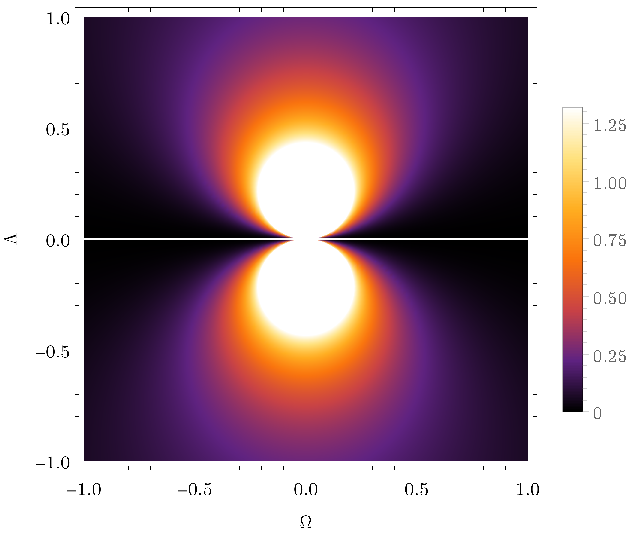
\includegraphics[scale=0.7]{../dp_text/img/2level_pla.pdf}
%   \end{figure}  

% }

% \frame{
%   \frametitle{Otázka oponenta ohledně Dvouhladinového systému}
%   \framesubtitle{Metrický tenzor $g_{01}$}
%   \begin{figure}[h]
%     \centering
%     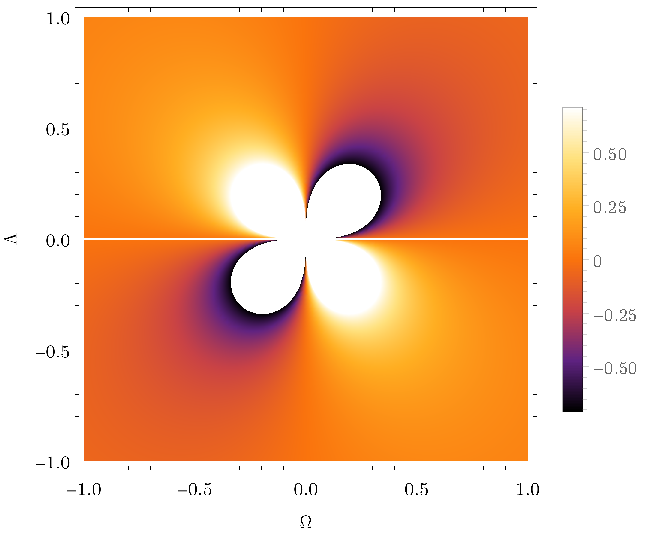
\includegraphics[scale=0.7]{../dp_text/img/2level_plb.pdf}
%   \end{figure}  

% }

% \frame{
%   \frametitle{Otázka oponenta ohledně Dvouhladinového systému}
%   \framesubtitle{Metrický tenzor $g_{11}$}
%   \begin{figure}[h]
%     \centering
%     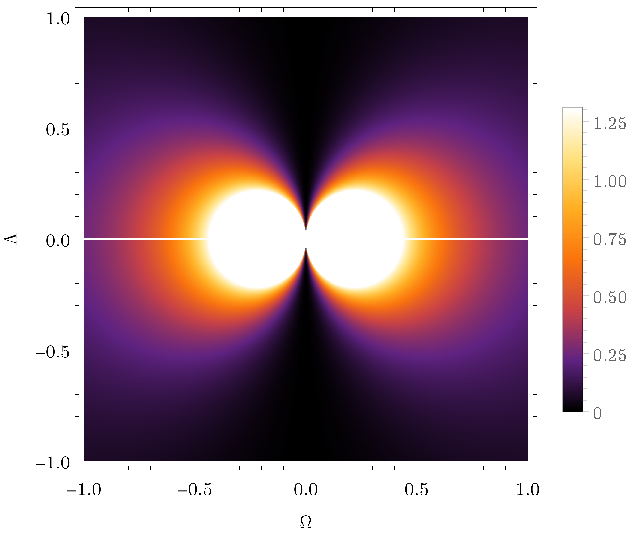
\includegraphics[scale=0.7]{../dp_text/img/2level_plc.pdf}
%   \end{figure}  

% }


\end{document}